\documentclass[10pt,twocolumn]{article}

\usepackage[letterpaper,margin=0.72in,columnsep=0.24in]{geometry}
\usepackage[T1]{fontenc}
\usepackage{lmodern}
\usepackage{microtype}
\usepackage{amsmath,amssymb}
\usepackage{booktabs}
\usepackage{graphicx}
\usepackage{float}
\usepackage[skip=2pt]{caption}
\usepackage{xcolor}
\usepackage{tikz}
\usetikzlibrary{arrows.meta,positioning,fit,calc}
\usepackage[round,authoryear]{natbib}
\usepackage{hyperref}
\hypersetup{colorlinks=true,linkcolor=blue,citecolor=blue,urlcolor=blue}
\setlength{\textfloatsep}{5pt plus 1pt minus 2pt}
\setlength{\floatsep}{4pt plus 1pt minus 2pt}
\setlength{\intextsep}{5pt plus 1pt minus 2pt}
\captionsetup[table]{position=top,skip=2pt}

\title{When LoRA Composition Fails: Capability Retention Without Functional Composition}
\author{Nassim Berrada\\Unfolding Labs\\\texttt{nassim@unfoldinglabs.ai}}
\date{Preprint}

\begin{document}
\maketitle

\begin{abstract}
Parameter-space adapter merging is often discussed as a way to combine capabilities. A stronger claim is that a weighted merge of two independently trained LoRA adapters will execute an unseen transformation formed by applying task A followed by task B. We study this distinction with a controlled benchmark of deterministic structured-record transformations. The benchmark separates atomic competence, capability retention, dedicated composite training, joint training, and dynamic composition. Across five retained configuration families, dedicated composite adapters reach approximately 98--100\% IID accuracy, while additive and CAT dynamic composites remain at 0\% on the analyzed composite evaluations. Atomic retention varies substantially, so dynamic failure is not reducible to complete destruction of one constituent capability. Stored-adapter analysis finds attention-only updates and no simple relationship between update cosine similarity and functional composition. The result is a boundary condition: capability coexistence does not imply functional composition. We release the benchmark, predictions, qualification reports, and analysis utilities to support further study of adapter interference and ordered execution.
\end{abstract}

\section{Introduction}

Low-rank adapters make it inexpensive to specialize a shared model and attractive to reuse those specializations together. A natural experiment is to train an adapter for task A, train another for task B, merge them, and test a new prompt requiring both transformations. This experiment tests more than multitask retention. It tests whether a parameter-space operation can realize a new computation that neither adapter was trained to perform alone.

The distinction matters because an additive merge has the form
\begin{equation}
    \Delta W_{\mathrm{merge}} = \alpha \Delta W_A + \beta \Delta W_B,
\end{equation}
whereas sequential task execution requires an ordered computation. In general, the former is not the latter. A merged model may retain responses to A and B prompts while failing a prompt that asks for A followed by B.

We investigate this failure mode in a small, controlled setting. Inputs are key--value records and tasks are deterministic transformations such as sorting fields, selecting values, normalizing values, removing duplicates, renaming fields, and swapping keys and values. This setting makes the target program explicit and allows evaluation beyond string formatting.

Our contributions are:
\begin{itemize}
    \item a qualification protocol separating atomic task validity from composition success;
    \item a controlled comparison of dedicated composite adapters, joint controls, additive merges, and CAT merges;
    \item an analysis of capability retention, interference, and stored LoRA update geometry; and
    \item a reproducible benchmark and diagnostic toolkit for studying when adapter merging preserves capabilities without composing them.
\end{itemize}

The paper does not claim that LoRA merging is generally ineffective. It reports a systematic boundary observed for independently trained adapters, structured transformation prompts, and the merge mechanisms evaluated here.

\section{Research question}

An \emph{atomic task} is a single deterministic transformation learned and evaluated on its own, such as sorting fields or selecting values. A \emph{composed task} is a new target formed by applying two such transformations in a specified order. The order matters whenever the first transformation changes the record seen by the second. A \emph{dynamic adapter} is assembled at inference time from independently trained constituent adapters and has not been trained on the composed target. By contrast, a \emph{dedicated adapter} is trained directly on composed examples and provides a learnability control.

The central question is whether a parameter-space combination can produce the behavior of an ordered composite that is absent from both constituent training sets. This question is distinct from whether the combination retains useful responses to the constituent prompts. We call that latter property \emph{atomic retention}; the loss relative to standalone performance is \emph{interference}. \emph{Functional composition} means solving the unseen ordered target, whereas \emph{sequential execution} is a different mechanism that explicitly preserves the intermediate computation.

The study therefore asks: under what task relationships and adapter interactions can independently trained LoRA updates coexist without destroying constituent behavior, and when---if ever---does that coexistence amount to functional composition? Additive and CAT merges provide the static parameter-space cases examined here; dedicated and joint controls establish whether the target itself is learnable.

\section{Related Work}

Several strands of work motivate adapter composition, but they do not all make the same operational claim. LoRA introduced low-rank updates as a parameter-efficient alternative to full fine-tuning \citep{hu_lora}. Task arithmetic combines task vectors to transfer or retain capabilities \citep{ilharco_task_arithmetic}, while model soups average fine-tuned models when their parameters are compatible \citep{wortsman_soups}. TIES-Merging addresses parameter interference through trimming, sign election, and merging \citep{yadav_ties}. AdapterFusion instead learns a composition module over task-specific adapters \citep{pfeiffer_fusion}. These methods all combine information from multiple adaptations, but they do not all promise that a fixed weighted sum will execute an ordered program.

Recent work is closer to the present question. LoRA Soups explicitly evaluates skill composition and reports strong results for concatenating LoRA updates on practical tasks \citep{prabhakar_lora_soups}. That work motivates testing composition rather than only multitask retention, while also leaving room for task-dependent failure modes. Other approaches use task-aware retrieval or learned routing to select and combine adapters \citep{adsul_task_aware,dhasade_lorouter,shah_molora}. These mechanisms can preserve task identity at inference time. Our additive and CAT experiments do not have such a router; they ask whether the static update itself contains the required composition.

Our experiment targets the strongest of these claims. It asks whether a static merge of two adapters can perform a transformation that requires both operations in a specified order, even though neither constituent adapter saw that composite target during training. A result that preserves A prompts and B prompts can support multitask coexistence without supporting this claim. A routing method might avoid the problem by selecting an adapter from task identity; a sequential method might avoid it by preserving the order of intermediate computation. We treat those as separate mechanisms rather than as alternative names for additive merging.

This distinction also changes what counts as a useful negative result. A zero score on an unseen composite prompt does not refute model merging as a way to combine capabilities. It does show that the particular merge operation, training setup, and task interface did not turn two task vectors into an ordered program. The controls in this paper are designed to make that narrower statement testable.

\section{Methodology}

The methodology is designed to make a narrow causal comparison possible. Every task uses the same deterministic record generator and structured schema, so differences can be attributed to task relation, merge operation, or adapter interaction rather than ambiguous targets. The evaluation combines controlled splits, independently trained constituent adapters, learnability controls, inference-time merges, and saved diagnostics. Figure~\ref{fig:controls} summarizes these elements; the subsections define the corresponding measurements.

\subsection{Data and splits}

Each task has 500 training examples, 200 validation examples, and 50 examples in each test split. The training set teaches the transformation and the validation set selects checkpoints. The IID test set uses held-out records from the same generator regime. The latent test set changes held-out properties such as field counts or value offsets while preserving the task rule. The composition-OOD split changes the composite target regime and directly tests the ordered two-operation program. These splits separate memorization of the record vocabulary from generalization of the transformation and from performance on an unseen composition.

\subsection{Atomic qualification}

An atomic adapter is trained and evaluated on one transformation, such as sorting fields or selecting values. We qualify each constituent before interpreting a merge. Qualification requires learning the atomic IID task, generalizing to the latent split, improving over the base model, and meeting per-seed stability checks. This prevents a failed constituent from being mistaken for composition interference. It also keeps dynamic success out of the qualification decision: failure of the merge is the observation being measured.

\subsection{Adapter training}

The base model is Qwen2.5-0.5B-Instruct. Each independent LoRA adapter uses rank 8, alpha 16, dropout 0.05, and targets the query, key, value, and output projections in the attention blocks. Training uses two epochs, AdamW, learning rate $2\times10^{-4}$, batch size 8, gradient accumulation of 2, and maximum sequence length 512. For every ordered pair, independent constituent adapters are trained separately. Dedicated composite and jointly trained controls use composite examples and the same model family and training schedule. These controls distinguish a failure of merging from a failure of the target, data, or prompt interface.

\subsection{Dynamic composition}

A dynamic adapter is assembled at inference time from independently trained adapters and receives no composite-task training. Additive composition forms a weighted sum of the effective LoRA updates, with weights $(0.25,0.75)$, $(0.5,0.5)$, and $(0.75,0.25)$ in the full sweep. CAT composition concatenates the low-rank factors so that the constituent updates occupy separate rank subspaces before the resulting update is applied. Both methods are static parameter-space operations: neither explicitly executes the first task, stores its intermediate record, or routes tokens to a task-specific adapter. Sequential and routed mechanisms therefore represent different hypotheses and are not treated as interchangeable with additive or CAT composition.

\subsection{Controls}

The base model establishes the prompt difficulty. Each constituent adapter is evaluated on the composite prompt to measure whether one task accidentally solves part of the target. The dedicated composite adapter is trained directly on the target, while the joint control uses composite data under the standard training procedure. Finally, the dynamic merge is evaluated on both composite prompts and atomic prompts. The atomic prompts measure retention; the composite prompts measure functional composition. A high dedicated score with a low dynamic score is the most direct evidence that the target is learnable but not produced by the merge.

\subsection{Evaluation}

The evaluator parses each prediction into structured fields and reports exact and structured metrics. When field order is not semantically required, it compares fields as multisets, so harmless reordering does not count as an error. It separately records parse failures, empty outputs, field counts, duplicate behavior, and operation-specific outcomes. The primary composite score is exact correctness of the required structured content on the unseen composite prompt. Atomic retention is reported on the two constituent prompts, and latent and composition-OOD results expose failures that an IID score can hide. Predictions and metadata are saved so that evaluation can be recomputed offline.

\subsection{Diagnostics and analysis}

The diagnostics layer checks that loading and applying an adapter does not mutate the stored weights, that repeated inference is deterministic, and that endpoint tests recover the expected behavior of each constituent adapter. It also joins predictions with parse and operation diagnostics. Stored safetensor weights are analyzed through effective updates $B A$, with global and module-local norms, cosine similarity, sign agreement, and high-magnitude overlap. The current adapters target attention projections only, so the module analysis records the absence of MLP and embedding updates rather than treating those groups as observed evidence.

\subsection{Qualification rule}

A reported configuration must pass the atomic learning and latent-generalization checks, the jointly trained composite control must solve the composite IID and latent splits, and adapter integrity, determinism, and endpoint checks must pass for every qualification seed. Dynamic success is not part of this rule. The purpose is to compare dynamic outcomes among task pairs for which the constituent tasks and the composite target are demonstrably learnable.

\begin{figure}[H]
\centering
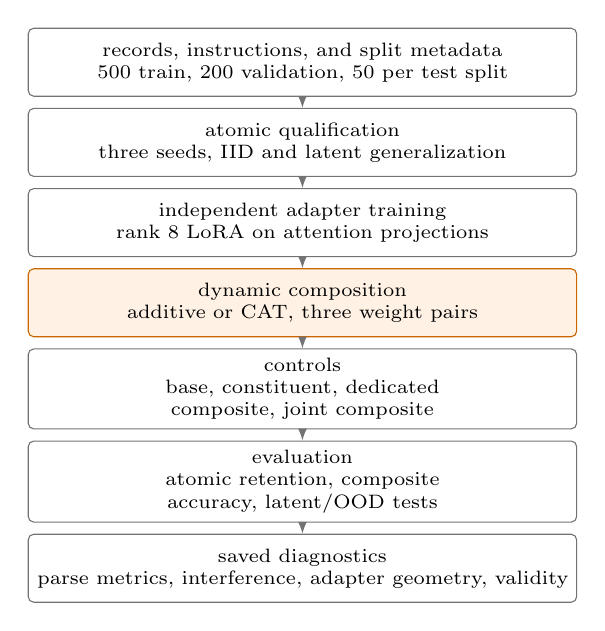
\begin{tikzpicture}[
  node distance=4pt,
  box/.style={draw=black!55, rounded corners=2pt, align=center, minimum height=0.34in, text width=2.65in, font=\scriptsize},
  focal/.style={box, draw=orange!80!black, fill=orange!10},
  arrow/.style={-{Latex[length=1.5mm]}, draw=black!55, line width=.45pt}
]
\node[box] (data) {records, instructions, and split metadata\\500 train, 200 validation, 50 per test split};
\node[box, below=of data] (atomic) {atomic qualification\\three seeds, IID and latent generalization};
\node[box, below=of atomic] (train) {independent adapter training\\rank 8 LoRA on attention projections};
\node[focal, below=of train] (merge) {dynamic composition\\additive or CAT, three weight pairs};
\node[box, below=of merge] (controls) {controls\\base, constituent, dedicated composite, joint composite};
\node[box, below=of controls] (eval) {evaluation\\atomic retention, composite accuracy, latent/OOD tests};
\node[box, below=of eval] (analysis) {saved diagnostics\\parse metrics, interference, adapter geometry, validity};
\draw[arrow] (data) -- (atomic);
\draw[arrow] (atomic) -- (train);
\draw[arrow] (train) -- (merge);
\draw[arrow] (merge) -- (controls);
\draw[arrow] (controls) -- (eval);
\draw[arrow] (eval) -- (analysis);
\end{tikzpicture}
\caption{The evaluation pipeline used in the study. Atomic qualification comes before composition, and the dedicated and joint controls separate target learnability from the behavior of an inference-time merge. The final analysis joins predictions with validity, retention, interference, and stored-adapter diagnostics.}
\label{fig:controls}
\end{figure}

\section{Results}

The study reports five retained experiment families: field renaming with key--value swap; field sorting with duplicate removal; field sorting with value normalization; field sorting with value selection; and the reverse value-selection/field-sorting order. The generated analysis contains 900 composition result rows across methods, weights, seeds, and splits.

\begin{table}[t]
\centering
\vspace{3pt}
\small
\caption{Split-wise mean performance across the five analyzed pair families, both dynamic methods, all weights, and all seeds. Dynamic and semantic scores coincide after multiset-aware structured evaluation. The selection--sorting contribution uses the controlled target generator.}
\label{tab:split-results}
\begin{tabular}{lrrr}
\toprule
Split & Dynamic & Semantic & Dedicated \\
\midrule
IID & 0.0\% & 0.0\% & 100.0\% \\
Latent & 0.0\% & 0.0\% & 99.2\% \\
Composition-OOD & 0.0\% & 0.0\% & 47.1\% \\
\bottomrule
\end{tabular}
\end{table}

\begin{table}[t]
\centering
\vspace{3pt}
\small
\caption{Mean atomic retention and interference on the IID split. Retention is composed accuracy divided by standalone accuracy. Interference is standalone accuracy minus composed accuracy. Values average both dynamic methods, all weights, and all seeds.}
\label{tab:retention}
\resizebox{\columnwidth}{!}{%
\begin{tabular}{lrrrr}
\toprule
Pair family & Ret. A & Ret. B & Int. A & Int. B \\
\midrule
Renaming--swap & 89.7\% & 77.7\% & 10.3\% & 22.3\% \\
Sorting--deduplication & 75.8\% & 80.0\% & 24.2\% & 20.0\% \\
Sorting--normalization & 73.7\% & 98.6\% & 26.3\% & 1.4\% \\
Sorting--selection & 80.6\% & 49.7\% & 19.4\% & 50.3\% \\
Selection--sorting & 49.7\% & 80.9\% & 50.3\% & 19.1\% \\
\bottomrule
\end{tabular}%
}
\end{table}

\paragraph{Result: Dedicated composite adapters learn the targets, while additive and CAT dynamic adapters do not.}

\paragraph{Evidence:} Dedicated adapters learn the composite task, but independently trained adapters do not dynamically realize it. Across the five analyzed pair families, additive and CAT methods score 0\% on the corrected composite evaluations, while dedicated and joint controls remain near-perfect where reported. The selection--sorting configuration also scores 0\% when its target requires both selection and a substantive reordering step.

\paragraph{Result: Dynamic failure is often asymmetric rather than a uniform loss of both skills.}

\paragraph{Evidence:} On the sorting--selection pair, the dynamic model retains approximately 81\% of sorting performance but only 50\% of value-selection performance on the IID split. Reversing the order changes the pattern: selection retention is approximately 50\%, while sorting retention is approximately 81\%. The composite score remains 0\% in both directions. The merged adapter can therefore favor one constituent behavior while failing to execute the ordered target. Composite accuracy alone would hide this distinction; the atomic-prompt controls expose which capability is being retained and which is being overwritten or suppressed.

The analyzed set also contains both orders for value selection and field sorting. Reversing the order changes which atomic capability suffers most, but it does not produce a positive dynamic result when the target requires both operations to change the record. This is a small test of order sensitivity, not a proof that every noncommutative pair behaves the same way. It does show why reporting one direction alone would hide an important part of the failure.

\paragraph{Result: Atomic retention and functional composition are separate outcomes.}

\paragraph{Evidence:} Atomic retention is asymmetric and pair-dependent. In sorting--selection, value-selection retention is approximately 49--51\%, while sorting retention is approximately 80\%. In the reverse order, the weaker component changes position but dynamic composition remains near zero. In renaming--swap, CAT retains approximately 91\% and 86\% on the two atomic prompts, yet composite accuracy remains 0\%. Thus, complete constituent destruction is not necessary for functional composition to fail.

These results separate two questions that are often conflated: whether a merged model still contains useful behavior, and whether it performs a new ordered program. The first can hold while the second fails.

The retained atomic behavior also gives a more useful failure description than a binary "merge failed" label. For sorting followed by selection, selection loses roughly half of its IID performance under the dynamic composite while sorting remains stronger. For the reverse order, the asymmetry flips with the adapter roles, yet the composite prompt remains unsolved. The merge can therefore contain recognizable fragments of the constituent skills without producing the intermediate representation required by the target program.

\paragraph{Result: Stored-update geometry does not provide a simple composition predictor.}

\paragraph{Evidence:} We extract LoRA tensors from the stored adapters and compare effective constituent updates on common modules. The current training configuration targets attention projections; no MLP adapter updates are present. Mean global/module cosine is approximately 0.16 for renaming--swap and sorting--selection, 0.23 for sorting--deduplication, and 0.39 for sorting--normalization. The highest-overlap retained pair nevertheless has 0\% dynamic accuracy.

Module-level cosine ranges from negative to strongly positive values within each pair. Sign agreement and high-magnitude overlap likewise vary by module. With only five retained pair families, these features are descriptive rather than predictive, but they rule out a simple hypothesis that higher update cosine is sufficient for functional composition.

The geometry should also be read with the target-module configuration in mind. The adapters update attention projections only, so the current measurements describe overlap in that subspace. They do not tell us whether an MLP update would preserve, overwrite, or route task-specific features. The absence of MLP updates is a limitation of the present experiment rather than evidence that MLP geometry is irrelevant.

\section{Discussion}

The central interpretation is not that LoRA merging is impossible. Rather, the experiment tests a stronger operation than many merging demonstrations require. Task-vector and model-merging results often target capability coexistence, transfer, or routing. A weighted sum can be useful for those goals without representing an ordered computation. Explicit routing or chaining may be required when task identity or intermediate representations must be preserved.

The negative result is therefore scientifically useful as a boundary condition. It shows that a dedicated composite control can solve the target while the parameter merge cannot, and that atomic retention is not an adequate proxy for compositionality. It also suggests that a useful predictor may need to describe where updates act and how they alter intermediate representations, rather than rely on a global vector angle alone.

\section{Limitations}

The study has a narrow scope. It uses Qwen2.5-0.5B-Instruct, one LoRA rank and scaling configuration, one family of structured-record tasks, and two primary parameter-space merge methods. The task vocabulary is synthetic and deliberately regular. That makes the target program and the validity checks clear, but it does not establish how the same behavior would appear in code, vision, natural-language reasoning, or larger models.

The number of retained pair families is also small. The five families cover useful differences in filtering, ordering, normalization, deduplication, renaming, and key/value transformation, yet they are not independent observations. Several share the same atomic adapters, and reverse-order experiments share the same pair geometry. Pair, seed, weight, and method are nested factors, so the current tables should not be used as if they were hundreds of independent samples.

The geometry features are limited by the saved adapter configuration. All current adapters target attention projections, and the global comparison flattens effective updates across common modules. That representation can hide layer-specific behavior, sign cancellation in the forward pass, and interactions with the frozen base model. The reported cosine values are therefore diagnostics, not mechanistic explanations.

Finally, explicit sequential composition remains underrepresented. A sequential adapter mechanism is not equivalent to generating an intermediate textual output and feeding it into a second model, and a failure of one implementation would not settle the question. The present results are strongest for additive and CAT merging.

\section{Future work}

Further work should change one factor at a time. A useful geometry extension would train matched adapters targeting attention and MLP projections, then compare layer-local conflict with atomic retention. A useful task extension would add a positive control whose operation is known to be compatible with a static merge, rather than adding more arbitrary transformations. A useful evaluation extension would compare a task router, explicit chaining, and parameter merging on the same examples. These experiments would make a stronger follow-up than another broad sweep over weights.

The retained corpus supports further study of the distinction between capability coexistence and functional composition. It also provides a compact evaluation dataset and diagnostic harness for comparing parameter-space merging with explicit execution and routing.

\section{Conclusion}

Across five retained structured-transformation pair families, additive and CAT LoRA merges preserved some constituent behavior in some settings but failed to implement the unseen ordered composite. Dedicated composite adapters solved the same targets, and update geometry did not yield a simple explanation based on cosine similarity. The appropriate conclusion is a distinction: capability coexistence is not functional composition.

The resulting benchmark provides task configurations, predictions, qualification reports, adapter tensors, and analysis scripts. These materials support direct comparison of parameter-space merging with explicit ordered execution and routing.

\appendix
\section{Appendix}

\subsection{Qualification thresholds}

Atomic qualification required mean IID accuracy of at least 0.75, mean latent accuracy of at least 0.60, an IID gain over the frozen base model of at least 0.15, IID and latent seed standard deviations no greater than 0.10, per-seed IID accuracy of at least 0.65, and per-seed latent accuracy of at least 0.50. Composite qualification required constituent accuracy on the composite prompt to remain at or below 0.40 on both IID and latent splits, joint and dedicated composite accuracy of at least 0.75 on IID data, and dedicated latent accuracy of at least 0.50. Adapter endpoint checks used an accuracy-difference tolerance of 0.001. Determinism and adapter-mutation checks were required to pass.

\subsection{Diagnostic analysis}

The stored diagnostics were grouped into four levels. Prediction diagnostics record parseability, empty outputs, predicted and target field counts, exact and multiset-aware content matches, duplicate predictions, content precision, recall, and F1. Operation diagnostics compare each prediction with the source record, the intermediate record, and the final target, both in order and as unordered pairs. Composition diagnostics summarize base, constituent, dynamic, dedicated, and joint accuracy together with composition gain and deficit. Adapter diagnostics inspect the saved LoRA tensors, form effective updates $B A$, and report tensor norms, parameter counts, module counts, global and module-local cosine similarity, sign agreement, high-magnitude overlap, and relative update norms. These measurements are joined by pair, method, seed, split, and weight so that output failures can be separated from retention loss and stored-update geometry.

\subsection{Task inventory}

The benchmark uses one input schema, a record containing ordered key--value fields. The atomic task registry contains the following transformations.

\subsection{Atomic tasks}

Every atomic adapter receives the same record schema, but each task changes one aspect of the record or its representation.
\begin{itemize}
    \item \textbf{Structured extraction.} Copies every key--value field. For example, \texttt{a: echo, b: hotel} remains unchanged.
    \item \textbf{Structured classification.} Inspects the record and returns a binary class such as \texttt{YES} or \texttt{NO} according to the task rule.
    \item \textbf{Field filtering.} Keeps fields at selected positions, such as the odd-positioned fields \texttt{a} and \texttt{c}.
    \item \textbf{Value selection.} Keeps fields whose values begin with a vowel, such as retaining \texttt{a: echo} while dropping \texttt{b: hotel}.
    \item \textbf{Field sorting.} Reorders fields by ascending value, so \texttt{b: alpha, a: echo} becomes \texttt{b: alpha, a: echo} regardless of input order.
    \item \textbf{Field reversal.} Reverses the input field order.
    \item \textbf{Duplicate removal.} Keeps the first occurrence of each value when multiple fields share a value.
    \item \textbf{Value normalization.} Lowercases each value, for example changing \texttt{Echo} to \texttt{echo}.
    \item \textbf{Field renaming.} Replaces keys with positional names such as \texttt{field\_1}, \texttt{field\_2}, and so on.
    \item \textbf{Key--value swap.} Exchanges the key and value in every pair, turning \texttt{a: echo} into \texttt{echo: a}.
    \item \textbf{Key prefixing.} Prepends \texttt{task\_} to each key, turning \texttt{a} into \texttt{task\_a}.
    \item \textbf{Key suffixing.} Appends \texttt{\_task} to each key, turning \texttt{a} into \texttt{a\_task}.
    \item \textbf{Value prefixing.} Prepends \texttt{value\_} to each value, turning \texttt{echo} into \texttt{value\_echo}.
    \item \textbf{Value suffixing.} Appends \texttt{\_value} to each value, turning \texttt{echo} into \texttt{echo\_value}.
\end{itemize}

\subsection{Atomic instruction prompts}

The following are the complete task instructions used by the atomic examples. In each prompt, \texttt{<record>} is replaced by the generated record, \texttt{<format>} is replaced by the selected output format, and \texttt{<answer>} marks the beginning of the expected answer. The optional noise prefix used by some splits is prepended to this instruction and does not change the task rule.
\begin{itemize}
    \item \textbf{Structured extraction.} \begin{quote}\small\ttfamily Extract every key-value field from the record. Return all fields and do not omit any field. Record: <record>. Format the answer as <format>. For ``lines'', output one ``key: value'' pair per line. For ``comma'', output ``key=value'' pairs separated by commas. Answer:\end{quote}
    \item \textbf{Structured classification.} \begin{quote}\small\ttfamily Classify the record as YES if at least one field value is exactly ``alpha''; otherwise classify it as NO. Record: <record>. Return exactly one label: YES or NO. Answer:\end{quote}
    \item \textbf{Field filtering.} \begin{quote}\small\ttfamily Filter the record by keeping only fields in odd-numbered positions: 1st, 3rd, 5th, and so on. Discard all even-numbered positions. Record: <record>. Format the answer as <format>. Answer:\end{quote}
    \item \textbf{Value selection.} \begin{quote}\small\ttfamily Select every field whose value begins with a vowel (A, E, I, O, or U). Discard all other fields. Record: <record>. Return the selected fields as comma-separated key=value pairs. If no field qualifies, return NONE. Answer:\end{quote}
    \item \textbf{Field sorting.} \begin{quote}\small\ttfamily Sort all fields alphabetically by their values in ascending order. Record: <record>. Format the answer as <format>. Preserve each key-value pair exactly. Answer:\end{quote}
    \item \textbf{Field reversal.} \begin{quote}\small\ttfamily Reverse the sequence of fields in the record from right to left, so the last field comes first and the first field comes last. Record: <record>. Format the answer as <format>. Answer:\end{quote}
    \item \textbf{Duplicate removal.} \begin{quote}\small\ttfamily Remove duplicate values from the record. Keep the first occurrence of each value and remove later fields having a value that has already appeared. Record: <record>. Return the remaining fields as comma-separated key=value pairs. Answer:\end{quote}
    \item \textbf{Value normalization.} \begin{quote}\small\ttfamily Normalize every field value by converting it to lowercase. Preserve all keys and all fields. Record: <record>. Format the answer as <format>. Answer:\end{quote}
    \item \textbf{Field renaming.} \begin{quote}\small\ttfamily Rename every field key using this mapping: the 1st field becomes field\_1, the 2nd field becomes field\_2, the 3rd field becomes field\_3, and so on. Preserve every value exactly. Record: <record>. Format the answer as <format>. Answer:\end{quote}
    \item \textbf{Key-value swap.} \begin{quote}\small\ttfamily Swap the key and value of each field in the record. Each original value becomes the key, and each original key becomes the value. Record: <record>. Format the answer as <format>. Answer:\end{quote}
    \item \textbf{Key prefixing.} \begin{quote}\small\ttfamily Add the fixed marker ``task\_'' before every field key. Record: <record>. Format the answer as <format>. Answer:\end{quote}
    \item \textbf{Key suffixing.} \begin{quote}\small\ttfamily Add the fixed marker ``\_task'' after every field key. Record: <record>. Format the answer as <format>. Answer:\end{quote}
    \item \textbf{Value prefixing.} \begin{quote}\small\ttfamily Add the fixed marker ``value\_'' before every field value. Record: <record>. Format the answer as <format>. Answer:\end{quote}
    \item \textbf{Value suffixing.} \begin{quote}\small\ttfamily Add the fixed marker ``\_value'' after every field value. Record: <record>. Format the answer as <format>. Answer:\end{quote}
\end{itemize}

\subsection{Composed tasks}

The composed generator applies two of these transformations in order and renders the resulting record in the same line or comma formats. The reported families are:
\begin{itemize}
    \item \textbf{Renaming--swap.} Renames the keys and then exchanges keys and values. An input \texttt{a: echo} first becomes \texttt{field\_1: echo}, after which the pair is swapped.
    \item \textbf{Sorting--deduplication.} Sorts fields by value and then removes repeated values. The second operation sees the sorted intermediate record.
    \item \textbf{Sorting--normalization.} Sorts by value and then lowercases the values.
    \item \textbf{Sorting--selection.} Sorts by value and then keeps only vowel-initial values.
    \item \textbf{Selection--sorting.} Keeps vowel-initial values and then sorts the retained fields by value. This reverses the previous order and tests whether the intermediate representation changes the result.
\end{itemize}

\begin{thebibliography}{99}
\small
\bibitem[Hu et al.(2022)Hu et al.]{hu_lora} Hu et al. \emph{LoRA: Low-Rank Adaptation of Large Language Models}. ICLR, 2022. arXiv:2106.09685.
\bibitem[Pfeiffer et al.(2021)Pfeiffer et al.]{pfeiffer_fusion} Pfeiffer et al. \emph{AdapterFusion: Non-Destructive Task Composition for Transfer Learning}. EACL, 2021. arXiv:2005.00247.
\bibitem[Wortsman et al.(2022)Wortsman et al.]{wortsman_soups} Wortsman et al. \emph{Model Soups: Averaging Weights of Multiple Fine-Tuned Models Improves Accuracy Without Increasing Inference Time}. ICML, 2022. arXiv:2203.05482.
\bibitem[Ilharco et al.(2022)Ilharco et al.]{ilharco_task_arithmetic} Ilharco et al. \emph{Editing Models with Task Arithmetic}. arXiv:2212.04089, 2022.
\bibitem[Yadav et al.(2023)Yadav et al.]{yadav_ties} Yadav et al. \emph{TIES-Merging: Resolving Interference When Merging Models}. NeurIPS, 2023. arXiv:2306.01708.
\bibitem[Prabhakar et al.(2024)Prabhakar et al.]{prabhakar_lora_soups} Prabhakar et al. \emph{LoRA Soups: Merging LoRAs for Practical Skill Composition Tasks}. arXiv:2410.13025, 2024.
\bibitem[Adsul et al.(2026)Adsul et al.]{adsul_task_aware} Adsul et al. \emph{Task-Aware LoRA Adapter Composition via Similarity Retrieval in Vector Databases}. arXiv:2602.21222, 2026.
\bibitem[Dhasade et al.(2026)Dhasade et al.]{dhasade_lorouter} Dhasade et al. \emph{Effective LoRA Adapter Routing using Task Representations}. arXiv:2601.21795, 2026.
\bibitem[Shah and Wagle(2026)Shah and Wagle]{shah_molora} Shah and Wagle. \emph{MoLoRA: Composable Specialization via Per-Token Adapter Routing}. arXiv:2603.15965, 2026.
\bibitem[Yadav et al.(2024)Yadav et al.]{det_tm} Yadav et al. \emph{Model Merging in the Era of Large Language Models}. arXiv:2403.13257, 2024.
\end{thebibliography}

\end{document}
